\input{../../preamble.tex}
% \bibliographystyle{plain} % Style BST file (bmc-mathphys, vancouver, spbasic).
% \bibliographystyle{unsrt} % Style BST file (bmc-mathphys, vancouver, spbasic).
\bibliography{pubs.bib}      % Bibliography 

\title{Professional Drone, Hybrid Power Pack  - Timebox 6}
\author{Team 2}

\begin{document}

\lstset{language=C,%
  % basicstyle=\color{red},
  breaklines=true,%
  morekeywords={matlab2tikz},
  keywordstyle=\color{blue},%
  morekeywords=[2]{1}, keywordstyle=[2]{\color{black}},
  identifierstyle=\color{black},%
  stringstyle=\color{mylilas},
  commentstyle=\color{mygreen},%
  showstringspaces=false,%without this there will be a symbol in the places where there is a space
  % numbers=left,%
  % numberstyle={\tiny \color{black}},% size of the numbers
  % numbersep=9pt, % this defines how far the numbers are from the text
  emph=[1]{for,end,break},emphstyle=[1]\color{red}, %some words to emphasise
  % emph=[2]{word1,word2}, emphstyle=[2]{style},    
}
% \lstdefinestyle{customc}{
%   belowcaptionskip=1\baselineskip,
%   breaklines=true,
%   frame=L,
%   xleftmargin=\parindent,
%   language=C,
%   showstringspaces=false,
%   basicstyle=\footnotesize\ttfamily,
%   keywordstyle=\bfseries\color{green!40!black},
%   commentstyle=\itshape\color{purple!40!black},
%   identifierstyle=\color{blue},
%   stringstyle=\color{orange},
% }

% \lstdefinestyle{customasm}{
%   belowcaptionskip=1\baselineskip,
%   frame=L,
%   xleftmargin=\parindent,
%   language=[x86masm]Assembler,
%   basicstyle=\footnotesize\ttfamily,
%   commentstyle=\itshape\color{purple!40!black},
% }

% \lstset{escapechar=@,style=customc}

\newcounter{udrboks}[section]\setcounter{udrboks}{0}
\renewcommand{\theudrboks}{\arabic{section}.\arabic{udrboks}}
\renewcommand{\theudrboks}{\arabic{udrboks}}
\newenvironment{udrboks}[2][]{%
  \refstepcounter{udrboks}%
  \ifstrempty{#1}%
  {\mdfsetup{%
      frametitle={%
        \tikz[baseline=(current bounding box.east),outer sep=0pt]
        \node[anchor=east,rectangle,fill=blue!20]
        {\strut Udregninger~\theudrboks};}}
  }%
  {\mdfsetup{%
      frametitle={%
        \tikz[baseline=(current bounding box.east),outer sep=0pt]
        \node[anchor=east,rectangle,fill=blue!20]
        {\strut Udregninger ~\theudrboks:~#1};}}%
  }%
  \mdfsetup{innertopmargin=10pt,linecolor=blue!20,%
    linewidth=2pt,topline=true,%
    frametitleaboveskip=\dimexpr-\ht\strutbox\relax
  }
  \begin{mdframed}[]\relax%
    \label{#2}}{\end{mdframed}}


\newcounter{formelboks}[section]\setcounter{formelboks}{0}
\renewcommand{\theformelboks}{\arabic{section}.\arabic{formelboks}}
\renewcommand{\theformelboks}{\arabic{formelboks}}
\newenvironment{formelboks}[2][]{%
  \refstepcounter{formelboks}%
  \ifstrempty{#1}%
  {\mdfsetup{%
      frametitle={%
        \tikz[baseline=(current bounding box.east),outer sep=0pt]
        \node[anchor=east,rectangle,fill=blue!20]
        {\strut Formler~\theformelboks};}}
  }%
  {\mdfsetup{%
      frametitle={%
        \tikz[baseline=(current bounding box.east),outer sep=0pt]
        \node[anchor=east,rectangle,fill=blue!20]
        {\strut Formler ~\theformelboks:~#1};}}%
  }%
  \mdfsetup{innertopmargin=10pt,linecolor=blue!20,%
    linewidth=2pt,topline=true,%
    frametitleaboveskip=\dimexpr-\ht\strutbox\relax
  }
  \begin{mdframed}[]\relax%
    \label{#2}}{\end{mdframed}}

\newcounter{konstboks}[section]\setcounter{konstboks}{0}
\renewcommand{\thekonstboks}{\arabic{section}.\arabic{konstboks}}
\newenvironment{konstboks}[2][]{%
  \refstepcounter{konstboks}%
  \ifstrempty{#1}%
  {\mdfsetup{%
      frametitle={%
        \tikz[baseline=(current bounding box.east),outer sep=0pt]
        \node[anchor=east,rectangle,fill=green!20]
        {\strut Konstanter~\thekonstboks};}}
  }%
  {\mdfsetup{%
      frametitle={%
        \tikz[baseline=(current bounding box.east),outer sep=0pt]
        \node[anchor=east,rectangle,fill=green!20]
        {\strut Konstanter~\thekonstboks:~#1};}}%
  }%
  \mdfsetup{innertopmargin=10pt,linecolor=green!20,%
    linewidth=2pt,topline=true,%
    frametitleaboveskip=\dimexpr-\ht\strutbox\relax
  }
  \begin{mdframed}[]\relax%
    \label{#2}}{\end{mdframed}}
\pgfplotstableread[row sep=\\,col sep=&]{
  ide & stemmer  \\
  Paraply & 9  \\
  Fjernbetjening & 7  \\
  iAdapt & 2 \\
}\mydata
% \setcounter{secnumdepth}{1}
\maketitle
\thispagestyle{empty}

\textbf{Deltagere:}
\begin{figure}[h]
  \centering
  % BEGIN RECEIVE ORGTBL delt
  \begin{tabular}{|p{5cm}p{10cm}|}
    \hline
    &\\
    Stud. nr: 201602094 & Navn: Søren Holm Korsgaard \\
    \hline
    &\\
    Stud.nr.: 201607563 & Navn: Jacob Gustafsson \\
    \hline
    &\\
    Stud.nr.: 201704859 & Navn: Jonas Buus \\
    \hline
    &\\
    Stud.nr.: 20084327 & Navn: Simon Rasmussen \\
    \hline
    &\\
    Stud.nr.: 201704483 & Navn: Thomas Dueholm Jensen \\
    \hline
  \end{tabular}
  % END RECEIVE ORGTBL delt

\end{figure}
\vspace{-5mm}
% \clearpage
\setcounter{tocdepth}{2}
\tableofcontents
\thispagestyle{empty}
\newpage
% \pagenumbering{arabic}
\setcounter{page}{1}

% \section{Introduktion}
% \label{sec:introduktion}

\section{Strategy and planning (Søren, Jacob, Simon)}
\label{sec:strategy-planning}

\subsection{Ensretter (Søren)}
\label{sec:ensretter-soren}
Efter sidste timebox, hvor der blev beskrevet et krav til funktionaliteten af ensretteren. Det blev beskrevet at input spændingen skulle være minimum 9 volt i peak for at ensretteren kunne fungere. Derfor blev der opsat en måde som kunne teste motor og generator, med fokus på hvilken belastning og hvilke omdrejninger, der skal til for at generere 9 volt i peak. Dette var nødvendigt for at kunne komme videre med selve arbejdet på ensretteren. 

Dette stykke arbejde har sat ensretter arbejdet på standby, hvorfor der er blevet lavet ændringer i Development planen.

\subsection{Spændingsregulator (Jacob)}
\label{sec:spand-jacob}
% Grundet uventet tidlig barsel har spændingsregulatoren været lidt på pause. Det har givet en forsinkelse, og da jeg (Jacob) ikke har været kvik nok til at få bestilt de nødvendige komponenter hjem, har vi stået lidt i stampe med spændingsregulatoren.
Grundet uventet tidlig barsel er arbejdet med spændingsregulatoren forsinket, hvilket indebærer forsinket bestilling af komponenter.

% Derfor er det meste af denne timebox for spændingsregulatorens vedkommende gået op i ventetid. Denne ventetid er blevet brugt på rapportskrivning, således de frigivne ressourcer kan bruges på andre rapportelementer senere hen. 
Det betyder at spændingsregulatoren også kommer til at strække sig over næste timebox. I denne testes opstillingen af LM317.

\subsection{Motorstyring (Simon)}
\label{sec:motorstyring-simon}
Denne timebox beskriver designet af de tests som skal udføres for at specificere koefficienterne i PID-reguleringen. Næste timebox vil blive brugt på at realiserer disse tests.
% Analysen af PID regulering fra sidste timebox, har vi valgt at forsætte på, i henblik på at kunne opsætte en teststand, hvori vi kan aflæse nogle værdier. For at kunne estimere værdierne til PID reguleringen.   


\section{Design af teststand til analyse af PID (Simon)}
\label{sec:design-af-teststand}

Målet med dette afsnit er at give et udkast til en teststand som skal specificere koefficienterne $k_P$, $k_I$ og $k_D$ fra formlen:

\begin{equation}
  \label{eq:1}
  u(t)=k_Pe(t)+k_I \int_0^t e(\tau)\mathrm{d}\tau + k_D\frac{\mathrm{d}e(t)}{\mathrm{d}t}
\end{equation}

hvor $e(t)$ er fejl som funktion af tiden, $e(\tau)$ er fejl som funktion af den akkumulerede tid og $k_P$, $k_I$ og $k_D$ er koefficienter svarende til henholdsvis det proportionale, integrede og deriverede forhold.

I en teststand vil formålet være at test forskellige værdier af koefficienterne og i forskellige kombinationer. Målet med PID-reguleringen er at strømmen fra batteri til dronens propelmotorer er konstant. Tilgengæld skal spjældet til forbrændingsmotoren konstant reguleres. Derfor vil en teststand som udgangspunkt have følgende:
\begin{itemize}
\item input: strøm fra batteri til drone
\item output: regulering af spjæld via servomotor
\end{itemize}

Her vil $e(t)$ være et mål for forskellen mellem den ønskede strømstyrke og den faktiske.

Det er på nuværende tidspunkt ikke muligt at måle strømmen fra batteri til drone. For at lave en teststand som kan tjene som skabelon for senere tests fremstilles istedet en teststand som skal justere spjældet i forhold til motorens omdrejninger. Dvs:

\begin{itemize}
\item input: motorens omdrejninger
\item output: regulering af spjæld via servomotor
\end{itemize}

I dette tilfælde vil $e(t)$ være et mål for forskellen mellem det ønskede omdrejningstal og det faktiske.

For at få en grov ide niveauet af koefficienterne kan en simulink simulation være gunstig. I denne skal gøres en række antagelser af forholdet mellem spjældvinkel og omdrejningstallet. Når koefficienterne er tunet i simulink kan der laves en test.
\clearpage
I testen skal der laves forskellige trinsvise ændringer af omdrejningstallet. Fjare\autocite{pid1} har beskrevet hvordan 4 forskellige trinmønstre (se figur\ref{fig:paths}) blev brugt til at justere en PID-algoritme som blev brugt til en forbrændingsenhed i en ubemandet flyvende enhed.

\begin{figure}[h]
  \centering
  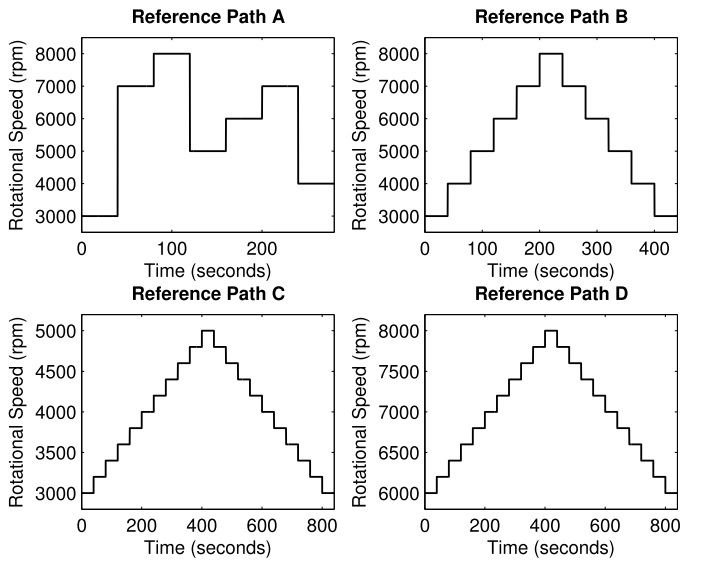
\includegraphics[width=0.7\textwidth]{refpaths.JPG}
  \caption{Trinmønstre}
  \label{fig:paths}
\end{figure}

På trods af at forbrændingsenheden altså ikke opladet batteri virker det relevant at tage udgangspunkt i lignende trinmønste til PID-kontrol af motoromdrejninger.

KL25 vil tjene både som microcontroller og datalogger. Som tidligere fremsat i timebox 5 kan et eksempel på PID-koden (fra Fjare\autocite{pid1}) være
\clearpage
\begin{lstlisting}[language=C,basicstyle=\ttfamily]
  void velPID ( ) {
    lowpassSpeed = alpha * lastLowpassSpeed + (1-alpha ) * measuredSpeed;
    K1 = kp * setpointWeight * (setpointSpeed-lastSetpointSpeed) + kp * (lastMeasuredSpeed-lowpassSpeed);
    K2 = ki * (setpointSpeed-lowpassSpeed);
    K3 = kd * (2 * lastMeasuredSpeed-lowpassSpeed-lastLastMeasuredSpeed);
    output = lastOutput-K1-K2-K3;
    throttlePos = floor(output + 0.5);
    if(throttlePos<throttleopen){
      output = (double) throttleopen;
      throttlePos=throttleopen;
    }
    if(throttlePos>throttlesafe){
      output = ( double )throttlesafe;
      throttlePos=throttlesafe;
    }
    lastLowpassSpeed = lowpassSpeed;
    lastLastMeasuredSpeed = lastMeasuredSpeed;
    lastMeasuredSpeed = lowpassSpeed;
    lastSetpointSpeed = setpointSpeed;
    lastOutput = output;
    throttle.writeMicroseconds(throttlePos);
  }
\end{lstlisting}


Følgende mangler og er målet for timebox 7:
\begin{itemize}
\item Tuning af koefficienterne i simulink.
\item Kode der skriver til \lstinline{TPM0->CONTROLS[PWM_CH_SERVO].CnV} med en spjældvinkel og som korrigeres af omdrejningstallet. Korrektionen skal foregå i rum tid hvor målet er et specifikt omdreningstal niveau forsøges opnået (fx 20 sekunder). Dvs. fx et for lopp der iterere gennem en liste af forskellige rpm-niveaur og for hvert niveau foretager PID-regulering i 20 sekunder.
\item En sensor som måler omdrejningstallet. Det er i gruppen diskuteret at tændspolen laver en gnist for hver omdrejning og at dette kan bruges som signal for omdrejningerne. Der skal bygges og kodes et setup.
\item Kode til logning af det opnåede samt det forsøgt opnåede omdrejningstal.
\end{itemize}
\clearpage
\section{Test af krav til ensretter (Thomas)}
\label{sec:test-af-krav}

Som beskrevet i timebox 5, afsnit 1 – Strategy and planning, er det valgt at sætte udviklingen af den aktive ensretter i bero, indtil der er foretaget en måling af spændingsniveauet på udgangen af generatoren ved tomgangsdrift. Dette skyldes, at den valgte IC (LT4320-1) til realiseringen af den aktive ensretter kræver et input på minimum 9 V (peak) (jf. datablad for LT4320-1\footnote{https://www.analog.com/media/en/technical-documentation/data-sheets/4320fb.pdf}) for at være funktionsdygtig. Vi er derfor nødt til at verificere, at generatoren til enhver tid vil producere minimum 9 V (peak). 

Der opstilles som følge af ovenstående konstatering et nyt krav til den aktive ensretter.\vspace{5mm}\\
\begin{tabular}[h]{ll}
  2.1.3.9&Der skal som minimum være 9 Volt (peak) på udgangen af generatoren,\\
           &inden denne tilkobles den aktive ensretter.\\
\end{tabular}
\vspace{2em}
\newline
For at verificere dette er der lavet et test setup, hvor det er muligt at måle outputtet (spænding) på én af generatorens tre faser. Test setuppet kan ses i nedenstående figur.

\begin{figure}[h]
  \centering
  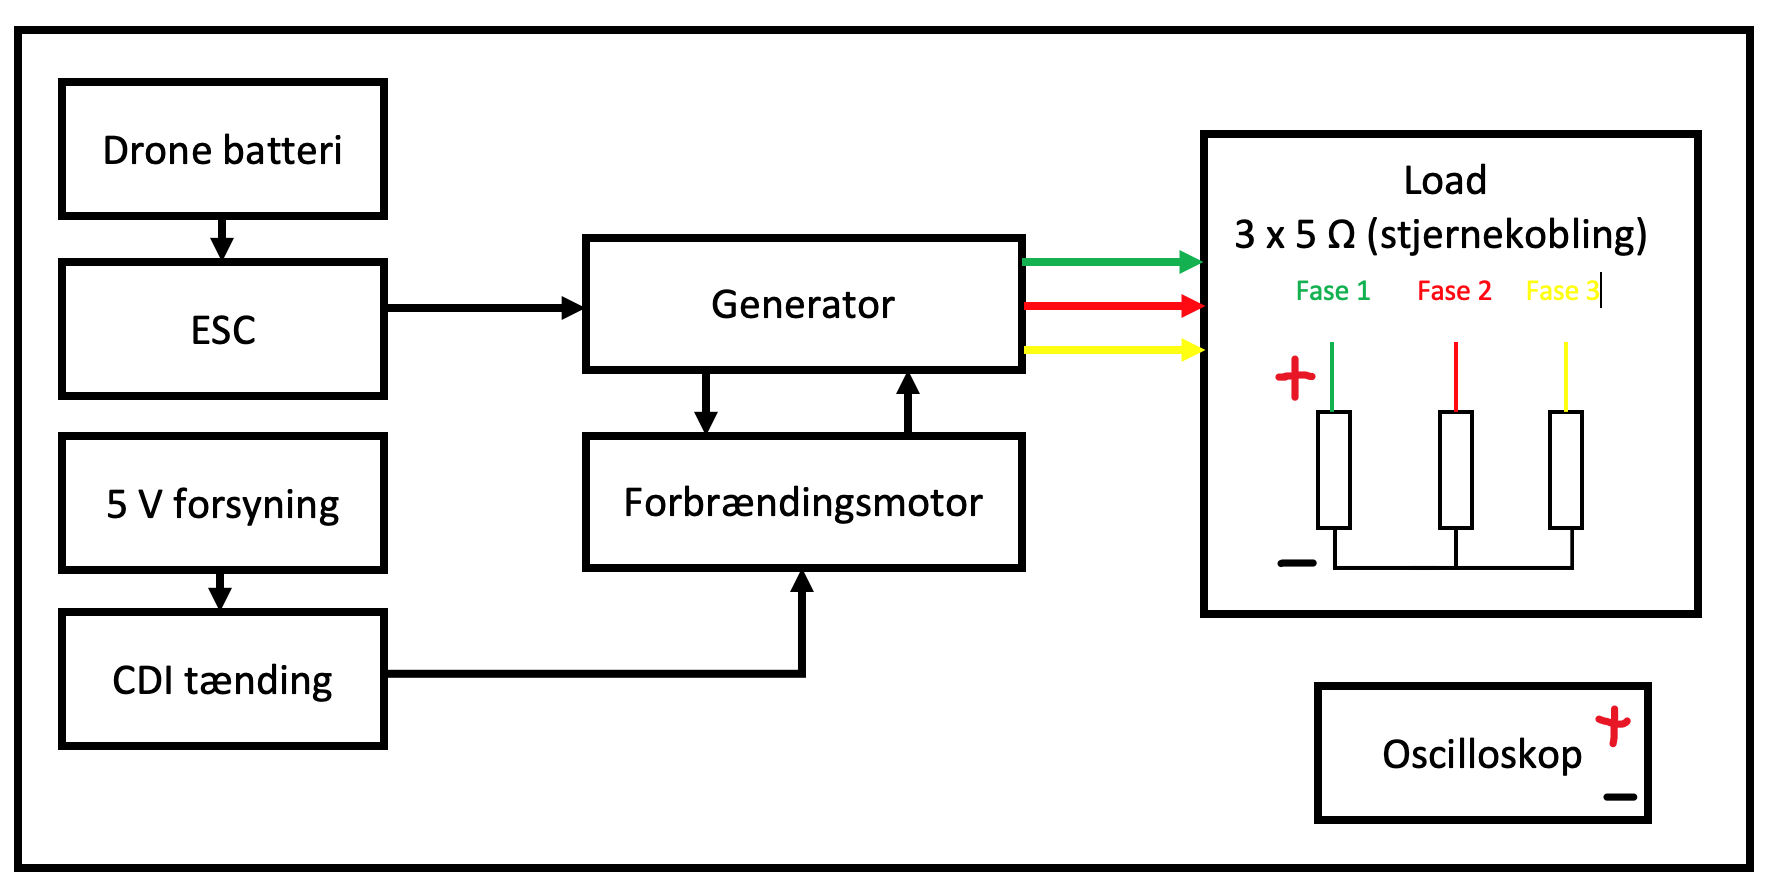
\includegraphics[width=0.45\textwidth]{blokdia.png}
  \caption{Blokdiagram over test setuppet}
  \label{fig:testsetup2}
\end{figure}


\begin{figure}[h]
  \centering
  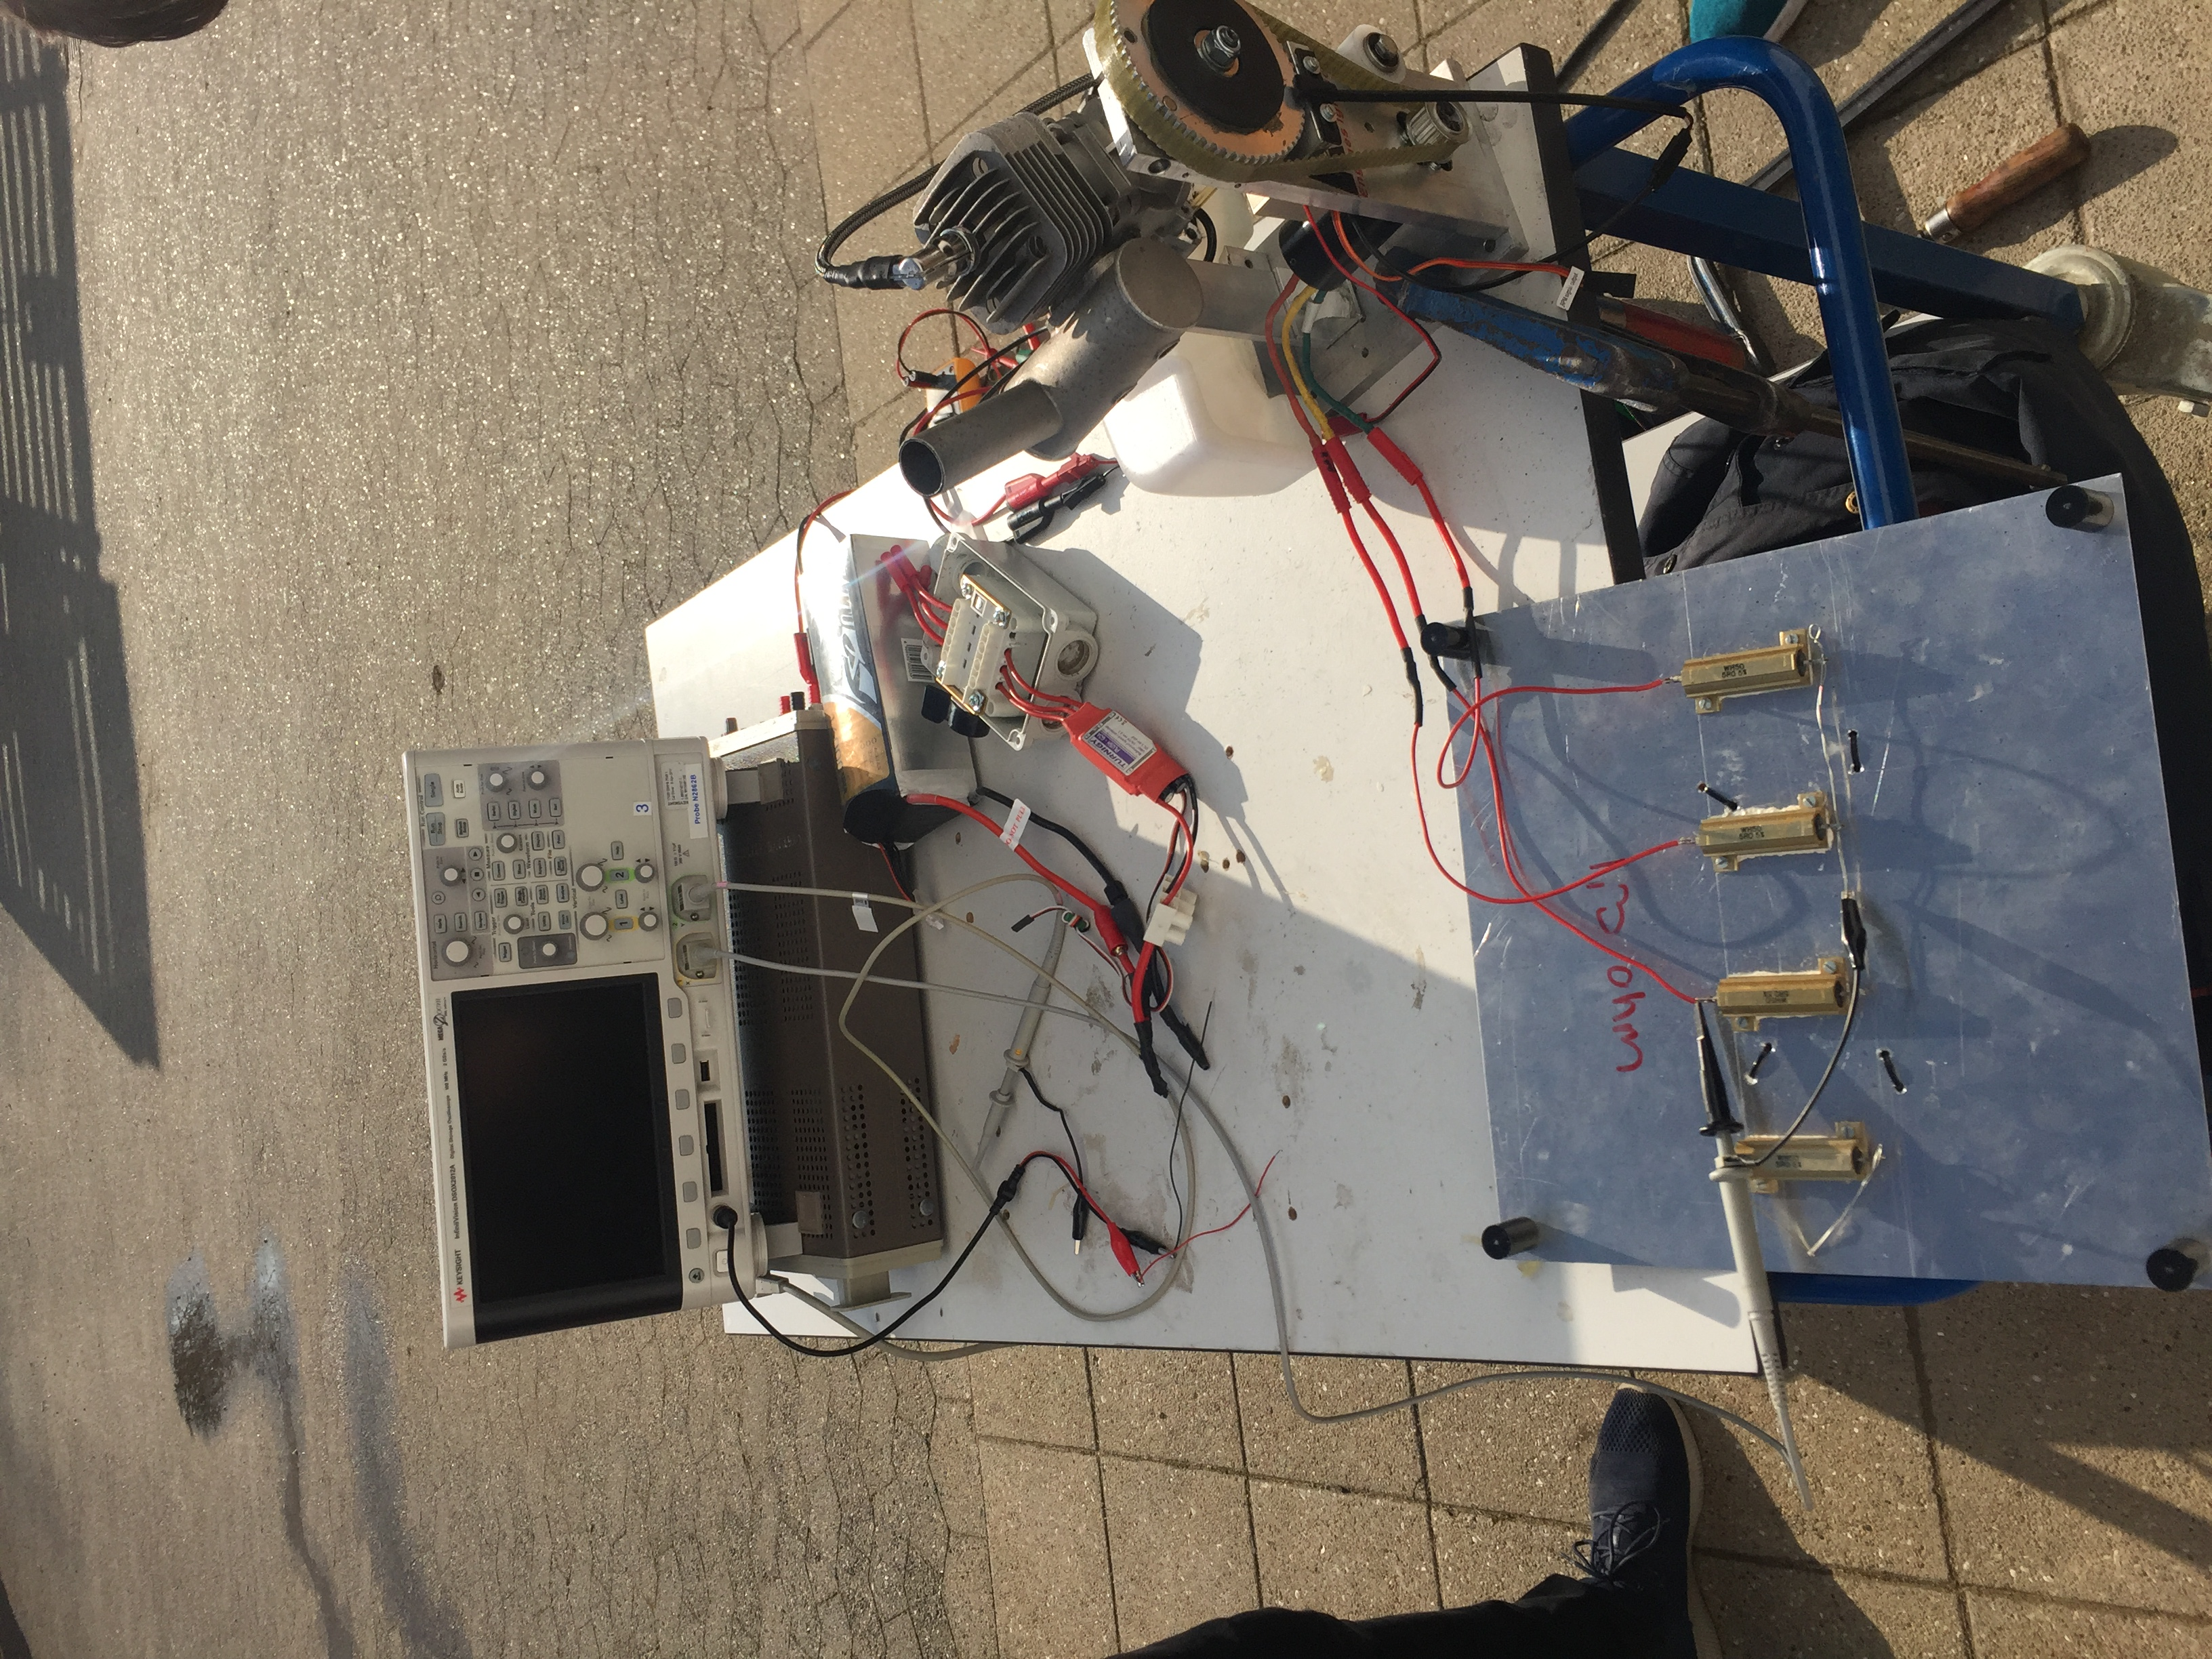
\includegraphics[width=0.45\textwidth]{testsetup.JPG}
  \caption{Foto af testsetup, hvor outputtet på én af generatorens faser måles med oscilloskop}
  \label{fig:testsetup}
\end{figure}


For at kunne foretage testen skal følgende komponenter/materialer bruges:
\begin{itemize}
\item Forbrændingsmotoren fra HPP, der via gearing på 3.75 er forbundet med generatoren.
\item Batteripakke fra DJI S1000 drone.
\item 5 Volt forsyning til CDI tændning.
\item ESC til opstart af generatoren (el-start af forbrændingsmotor).
\item Oscilloskop til generering af PWM signal til el-start, samt til måling af outputspænding over én af generatorens faser.
\item 3 stk. 5 $\omega$ effektmodstande opsat i stjernekobling.
\item Måleprobe tilkoblet oscilloskop.
\end{itemize}

Proceduren for testen vil være som følgende:

\begin{enumerate}
\item Tænd 5 Volts forsyningen til DCI tændningen.
\item Start forbrændingsmotoren vha. el-start (PWM signal fra oscilloskop med frekvens på 50 Hz og dutycycle på 1.25 ms sender ind i ESC’en).
\item Når forbrændingsmotor kører i tomgang, tilkobles generatorens tre faser til de tre 5 ohms effektmodstande i stjernekoblingen.
\item Tilkoble oscilloskopets måleprobe over én af de tre effektmodstande (se blokdiagram - figur~\ref{fig:testsetup2}).
\item Aflæs/gem graf over outputspændingen fra oscilloskopet.
\item Sluk forsyningen til CDI tændingen, hvorved forbrændingsmotor stopper.
\end{enumerate}

\begin{figure}[h]
  \centering
  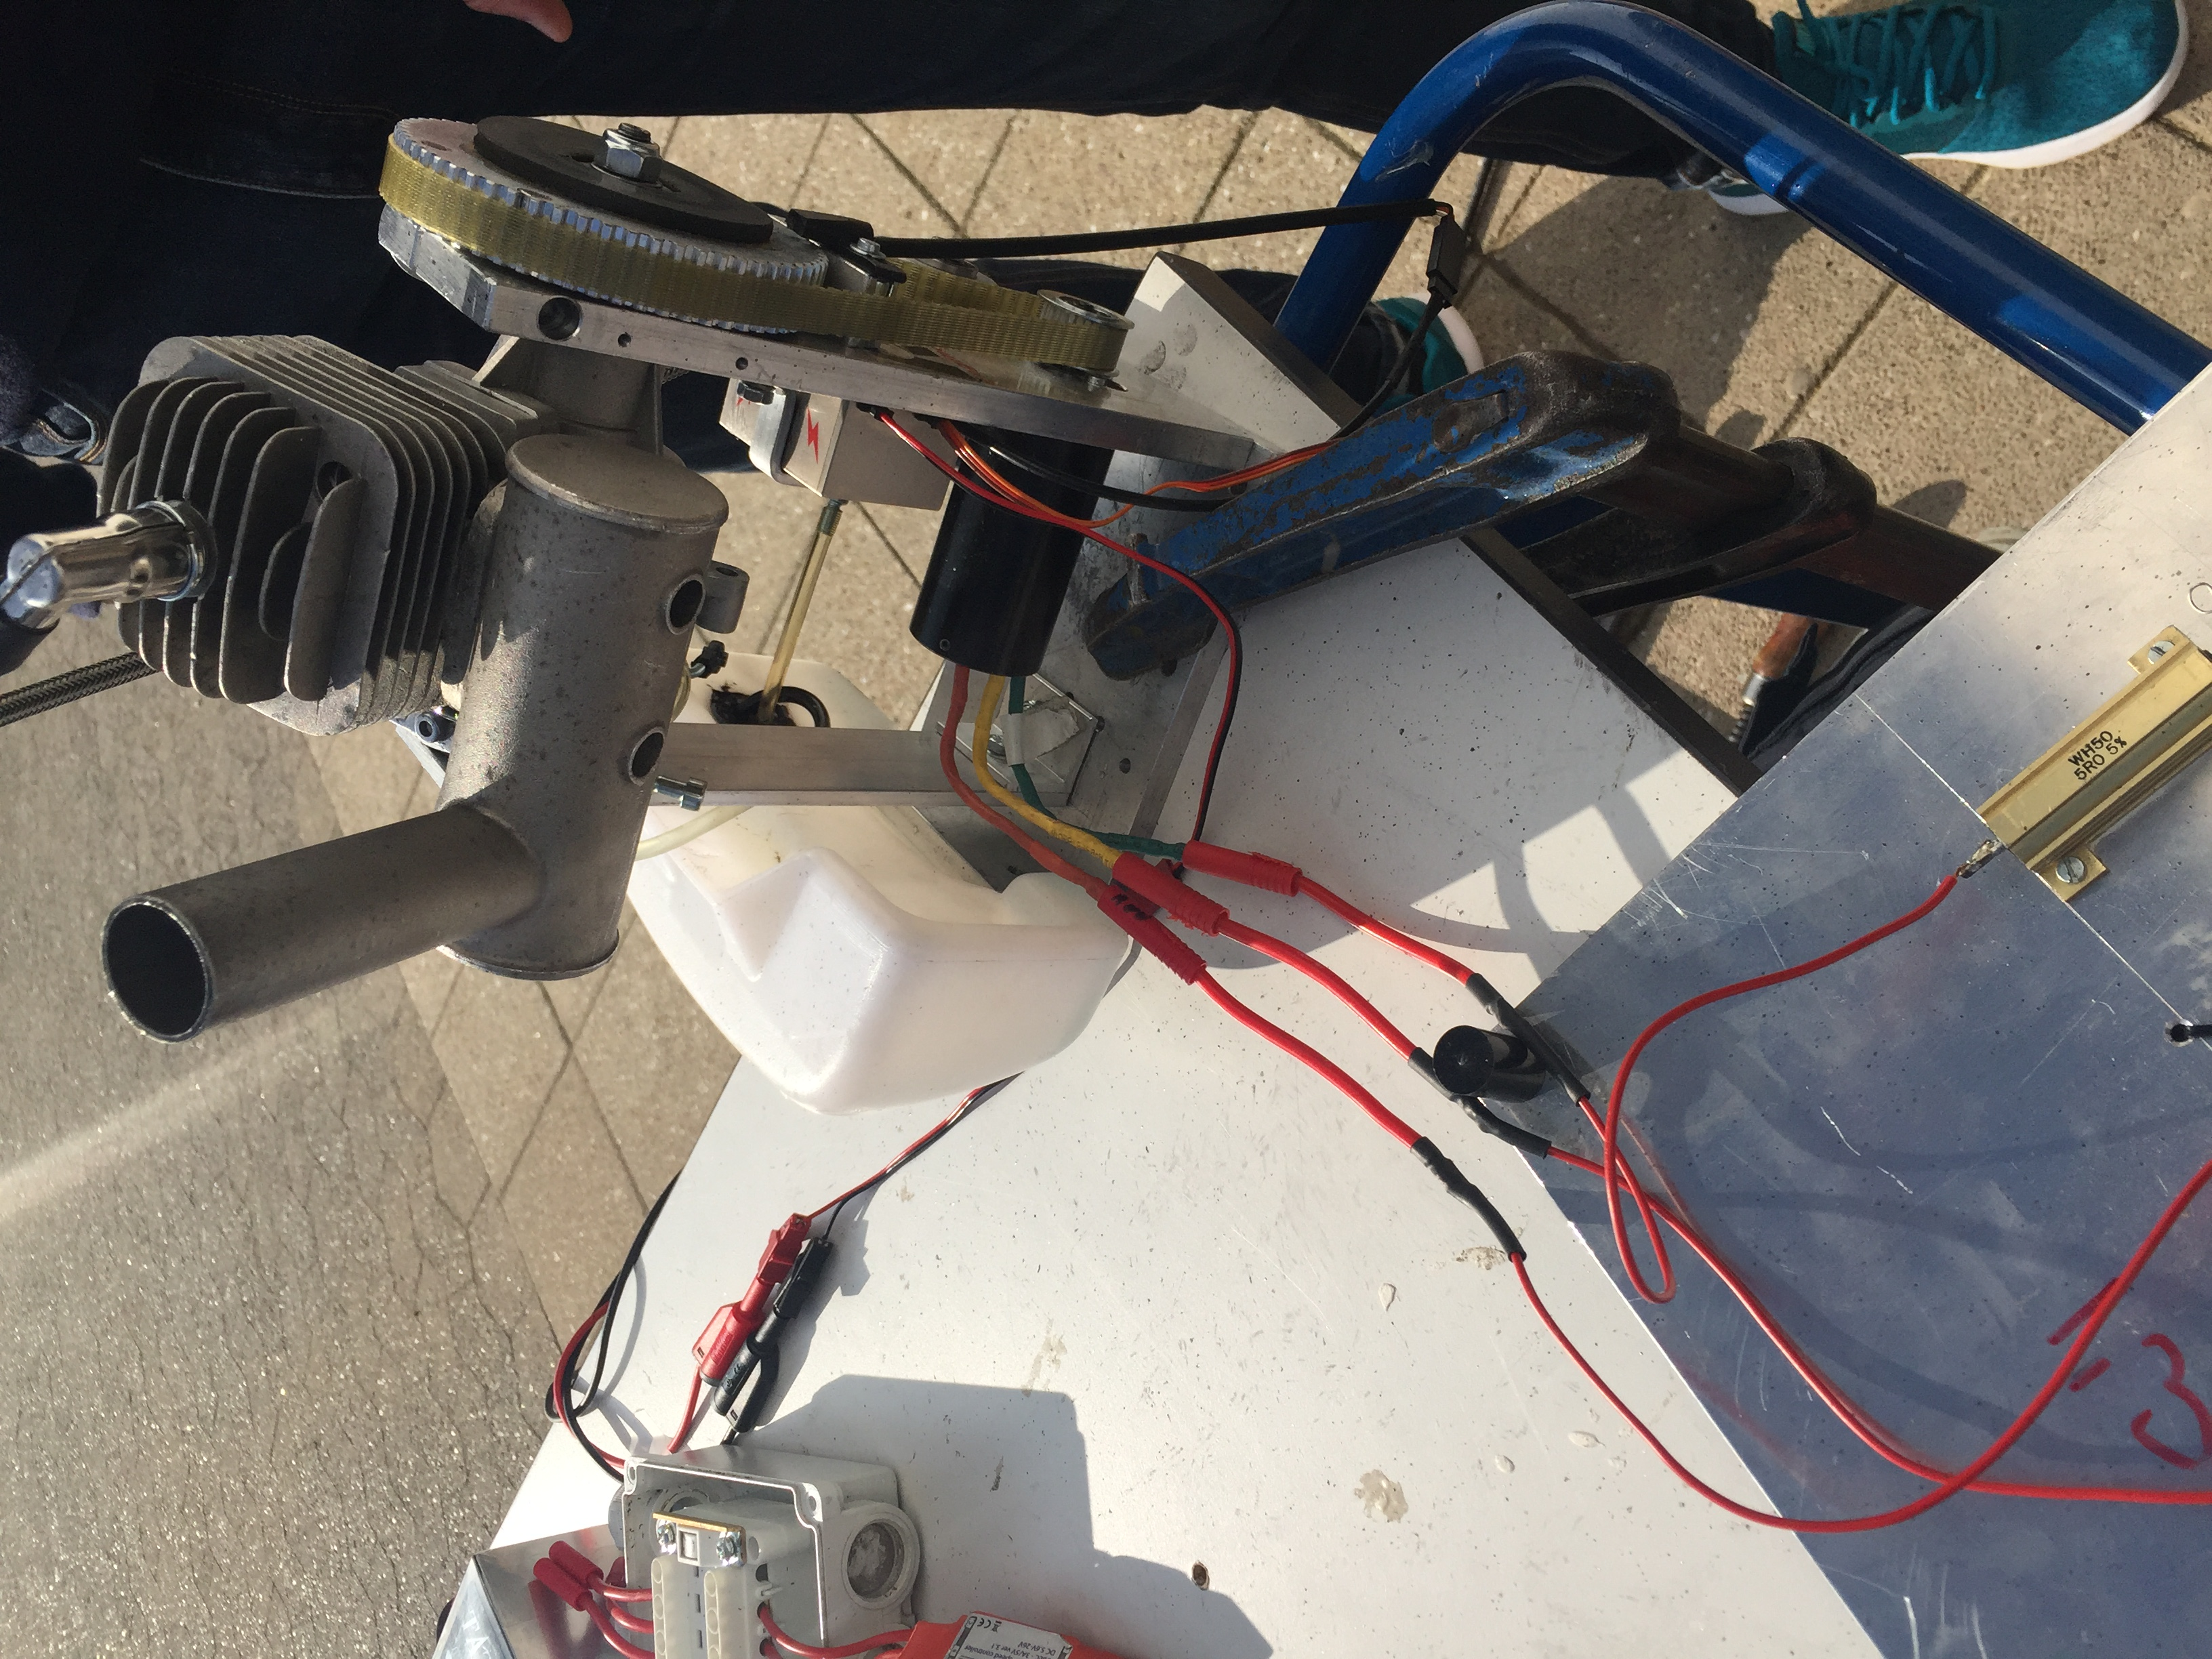
\includegraphics[width=0.45\textwidth]{testsetup2.JPG}
  \caption{Foto af sammenkoblingen af generator og load (3 x 5 $\omega$ effektmodstande i stjernekobling)}
  \label{fig:testsetup2}
\end{figure}

\begin{figure}[h]
  \centering
  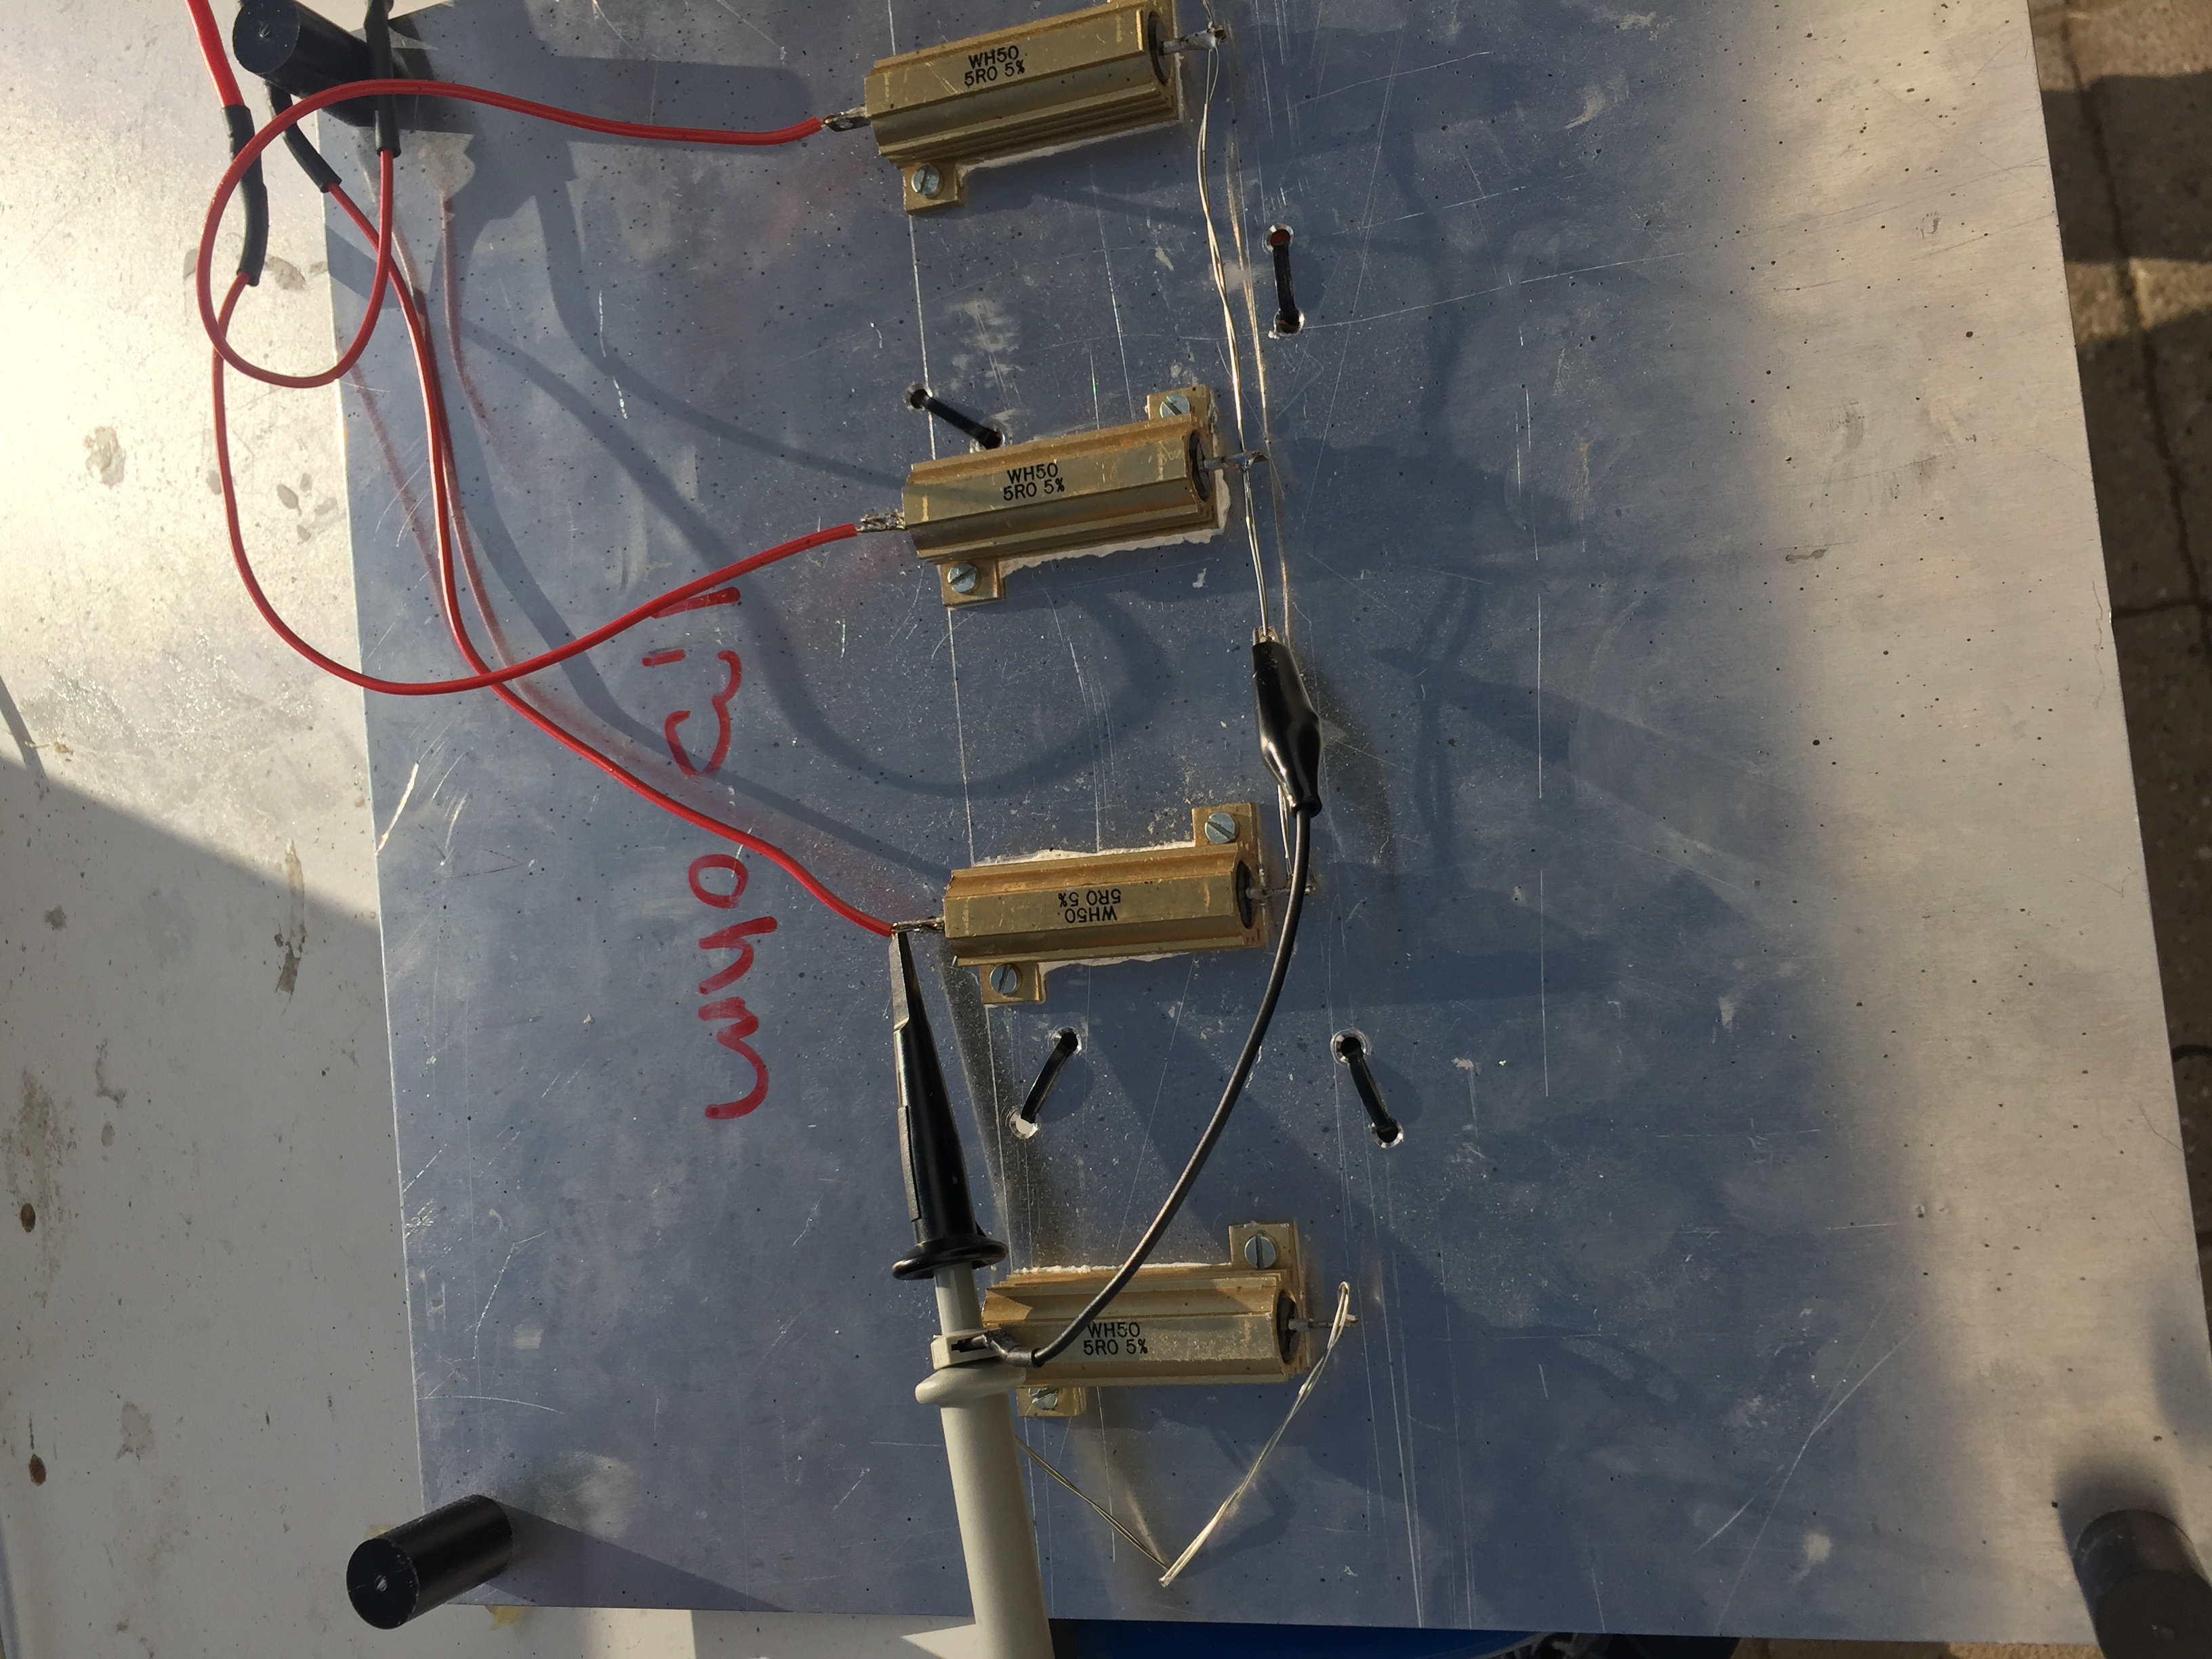
\includegraphics[width=0.45\textwidth]{loadstjernekobling.JPG}
  \caption{Foto af placering af måleprobe}
  \label{fig:testsetup2}
\end{figure}

Figur~\ref{fig:scope1} viser et skærmbillede af grafen for målingen af outputtet af én af generatorens tre faser.  
Som det ses, er der med forbrændingsmotoren kørende i tomgang en spænding på 11.4 Volt (peak) på udgangen af generatoren. 

\begin{figure}[h]
  \centering
  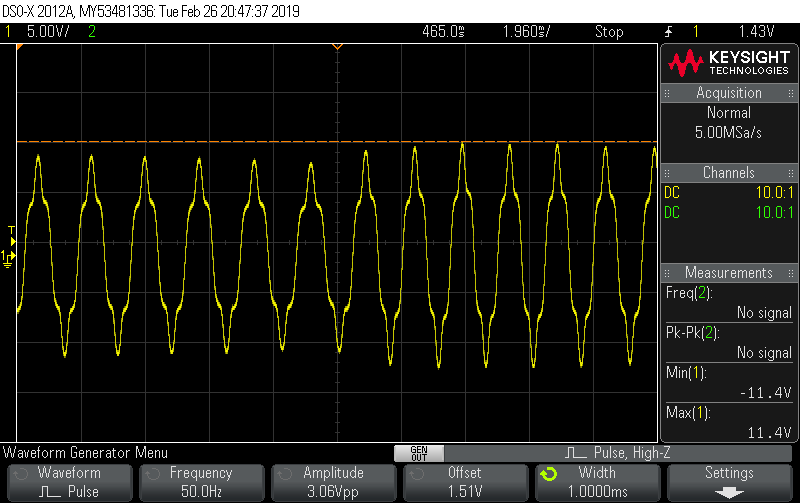
\includegraphics[width=0.45\textwidth]{scope0.png}
  \caption{Skærmbillede af graf over outputspændingen. (11.4 V peak)}
  \label{fig:scope1}
\end{figure}

% Når outputspændingen for tomgangsdrift kendes, vil det det nu være muligt at beregne, hvor mange rpm. forbrændingsmotoren kører med i tomgang.

\begin{equation}
  \label{eq:1}
  \mathrm{rpm}_{tomgang}=\frac{1400kv\cdot 11,4V}{3,75}=4256 \mathrm{rpm}
\end{equation}

% 4256 rpm. i tomgang er højt. Denne forhøjede tomgangsdrift i forbrændingsmotoren skyldes formentlig manglende inerti i svinghjulet (gearingen) samt den ekstra kraft det kræver at få generatoren til at rotere.

\subsection{Konklusion}
\label{sec:konklusion}

Som det ses ud fra resultatet af test setuppet, genereres et output på 11.4 Volt (peak) fra generatoren, når forbrændingsmotoren kører i tomgang. 

Da forbrændingsmotoren i drift altid som minimum vil køre i tomgang, kan det hermed konkluderes, at krav 2.1.3.9 er verificeret. 
\clearpage
\section{Spændingsregulatoren (Jacob)}
\label{sec:spandingsregulatoren}

\subsection{Structural analysis}
\label{sec:structural-analysis}

Som udgangspunkt er det valgt at gå videre med en BUCK-konverter som spændingsregulator. Imidlertid har der været en smule rod med bestillingen af komponenter, og dette bevirker, at der er kommet komponenter hjem til en spændingsregulator baseret på en LM317. Elementer der ellers var afbestilt. Men da komponenterne alligevel er tilgængelige, besluttedes det at teste dem op imod hinanden. Efter simuleringer fra tidligere timeboxes er det konkluderet, at begge typer burde opfylde requirements. Derfor opstilles der en række testkriterier:

\begin{enumerate}
\item Korrekt spænding
\item Tilstrækkelig strøm
\item Ripple
\item Driftsikkerhed og varmepåvirkning 
\item Pris og størrelse
\end{enumerate}

\subsection{Behavorial Design Test}
\label{sec:behav-design-test}

Nedenfor ses et diagram af systemet baseret på en LM317, som der arbejdes med i denne uge.

\begin{figure}[h]
  \centering
  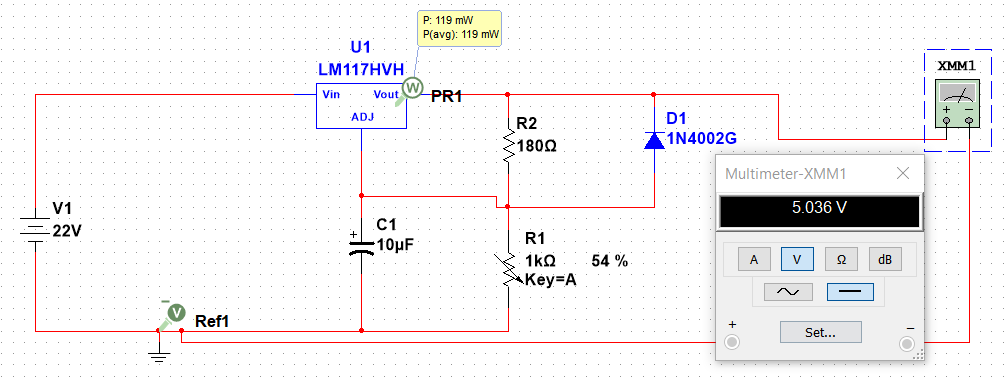
\includegraphics[width=0.65\textwidth]{srcirc.png}
  \caption{Diagram af systemet baseret på en LM317}
  \label{fig:srcirc}
\end{figure}
\clearpage
I figur~\ref{fig:srreal} ses opstillingen realiseret. Som det også ses af billedet har opstillingen en meget beskeden størrelse og vægt, hvilket er en stor fordel for vores vedkommende, som det også fremgår af de overordnede krav for projektet. Prisen på alle komponenter er billig. Det dyreste er LM317 til cirka 11 kroner stykket. Samlet pris for hele systemet beløber sig til cirka 19 kroner.

\begin{figure}[h]
  \centering
  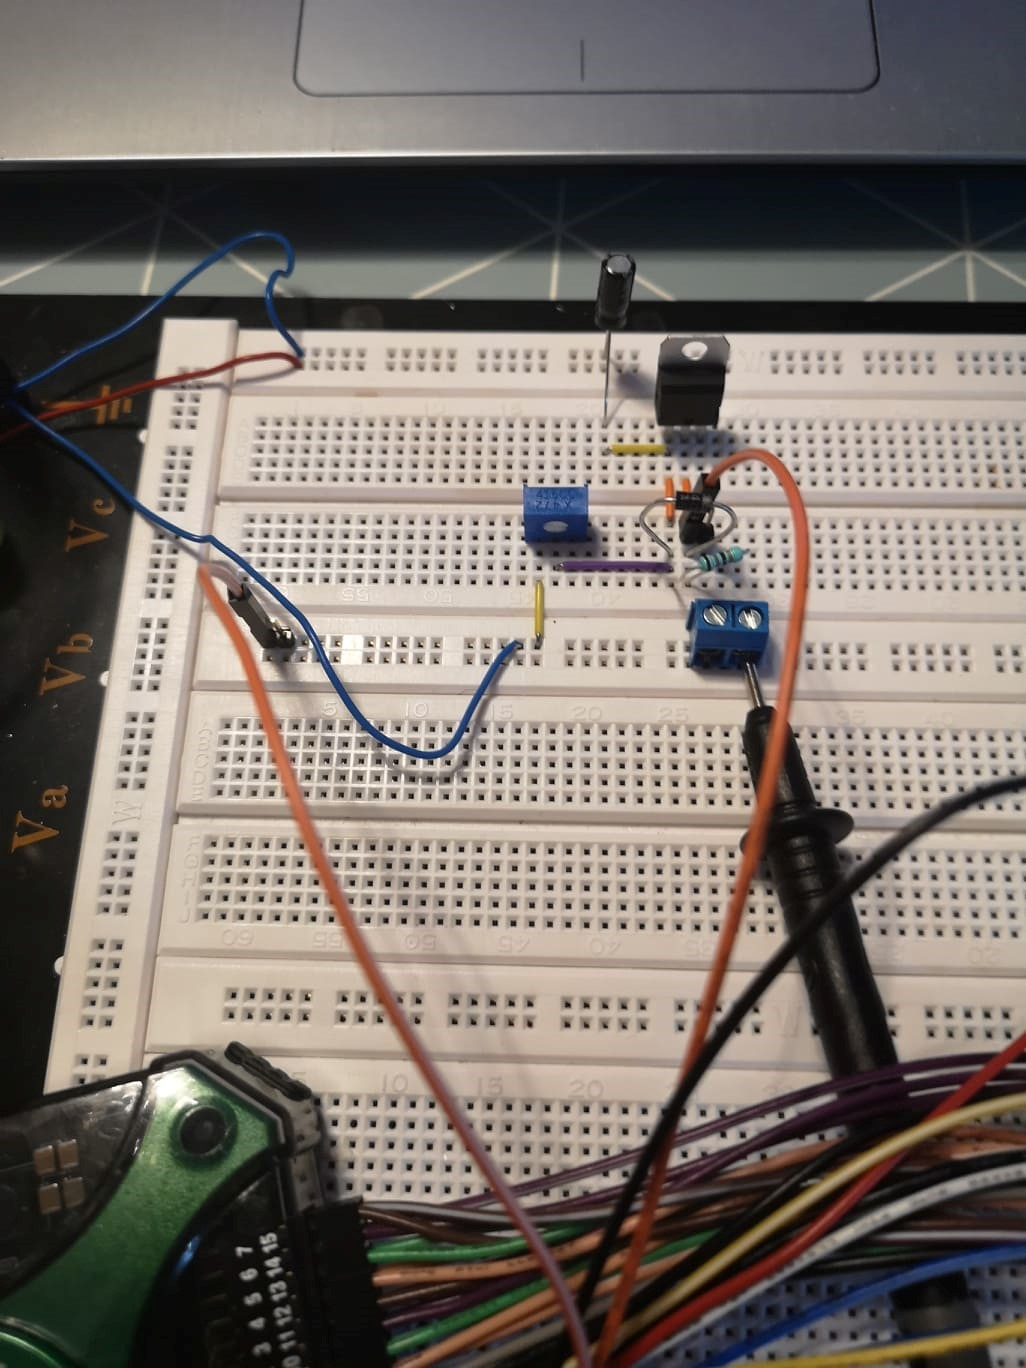
\includegraphics[width=0.32\textwidth]{srreal.jpg}
  \caption{Billede af realisering af opstillingen}
  \label{fig:srreal}
\end{figure}

Hernæst LM317 IC’en udsat for varme for at observere forskellene i spændingsniveauet (se figur~\ref{fig:varme}).

\begin{figure}[h]
  \centering
  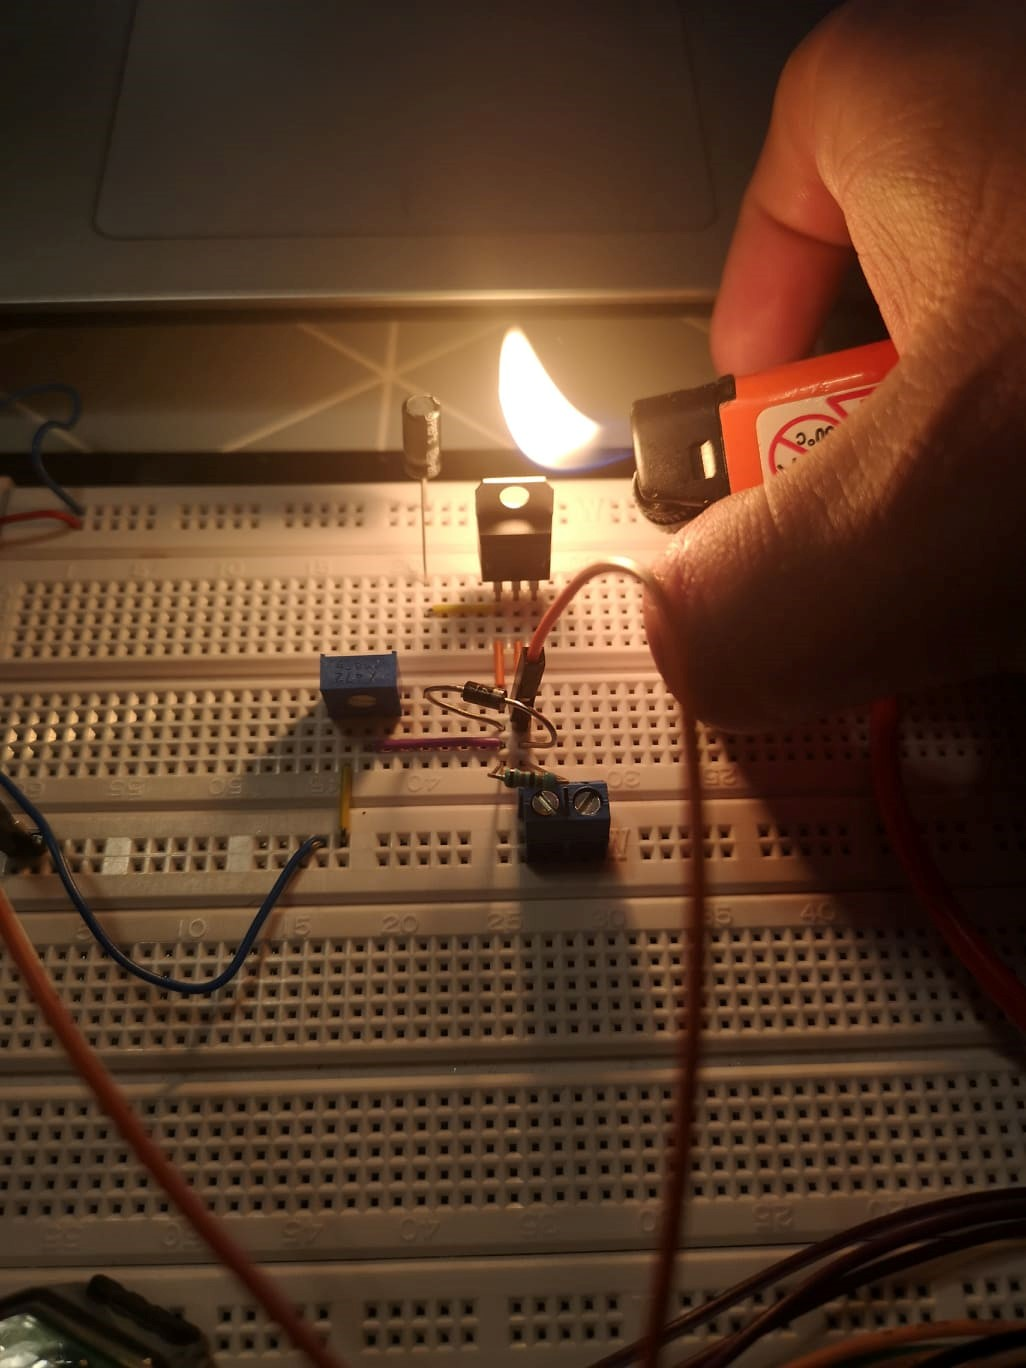
\includegraphics[width=0.32\textwidth]{varme.jpg}
  \caption{Varmetest}
  \label{fig:varme}
\end{figure}
\clearpage
\subsection{Testresultater}
\label{sec:testresultater}

På figur~\ref{fig:osc1} ses outputtet fra LM317-systemet. Som det ses, ligger spændingen lige omkring 5 V som påkrævet. Selvom der ikke er zoomet voldsomt meget ind, ses også et acceptabelt niveau af ripple. Potentiometeret blev udmålt til 538 $\Omega$, hvilket også stemmer meget godt overens med vores simulering. Der blev målt en strøm på 1024 mA på systemet, hvilket er en smule over det krævede niveau. Efter datasheetet burde vi kunne opnå 1,5 A.

\begin{figure}[h]
  \centering
  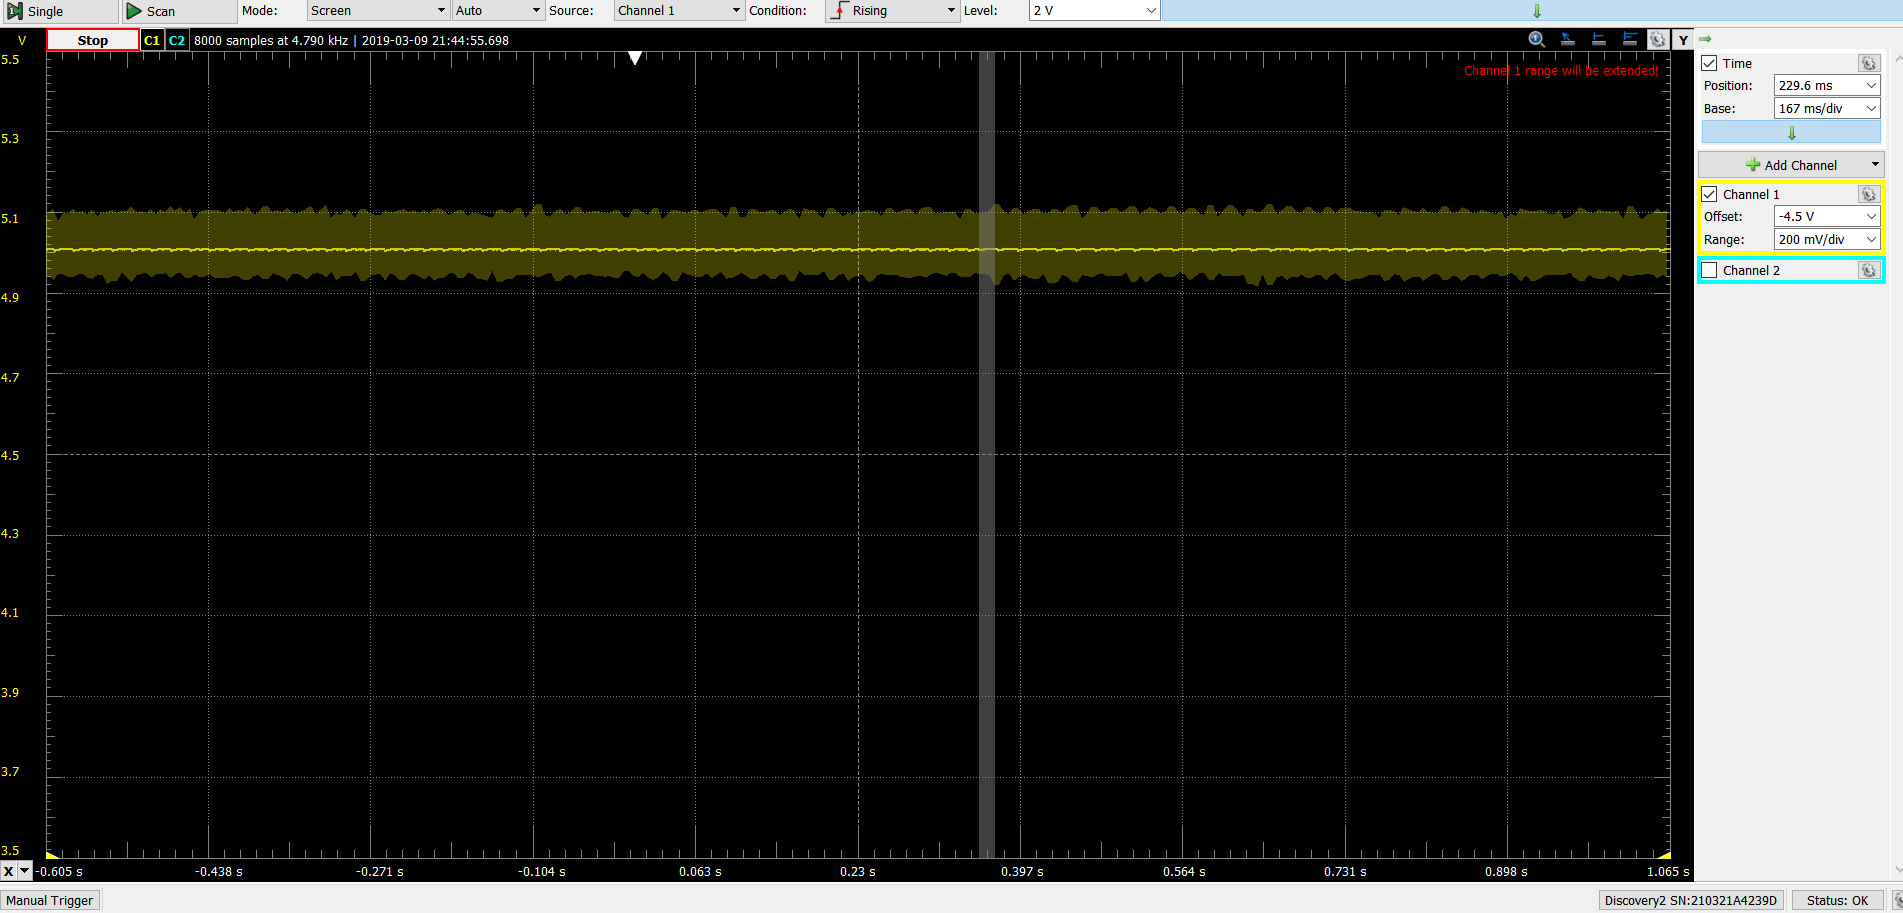
\includegraphics[width=0.55\textwidth]{osc1.png}
  \caption{Output fra LM317}
  \label{fig:osc1}
\end{figure}


Her ses spændingen efter det er udsat for lighteren i 30 sekunder. Spændingen falder en smule, men indenfor det acceptable, og ripple forøges ikke. 

\begin{figure}[h]
  \centering
  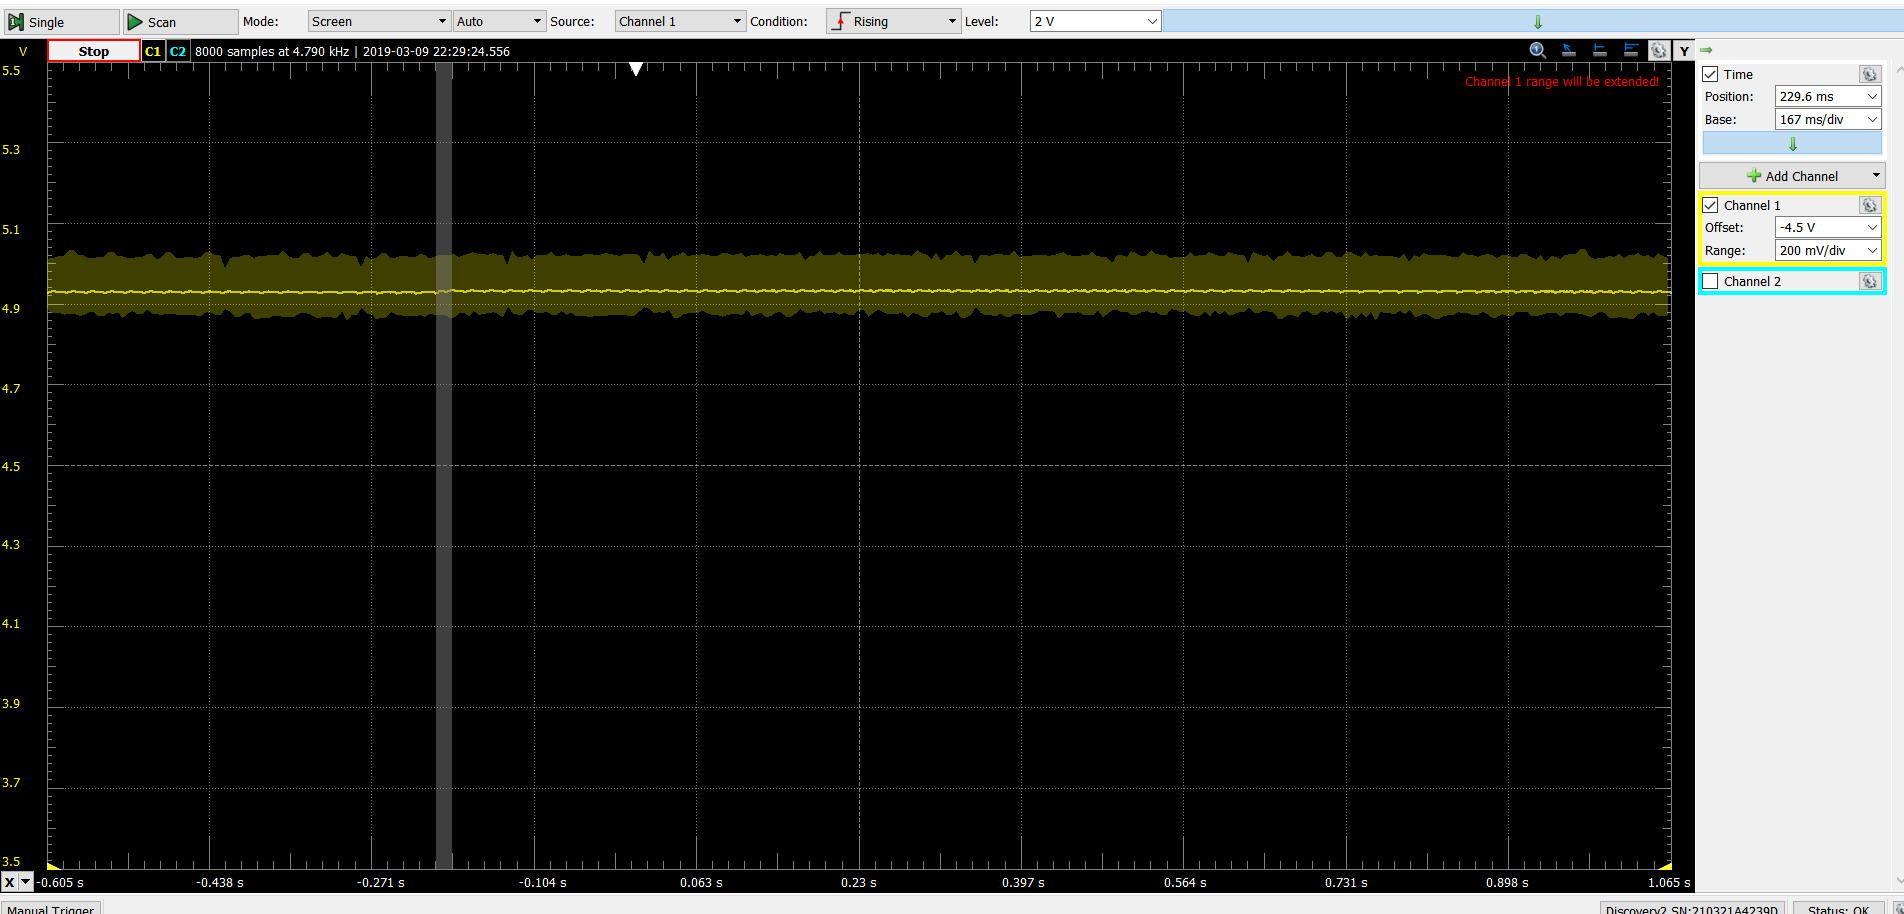
\includegraphics[width=0.55\textwidth]{osc2.png}
  \caption{Output fra LM317}
  \label{fig:osc2}
\end{figure}

\subsection{Konklusion}
\label{sec:konklusion-1}

Systemet lever op til alle krav. Sammenligning med TPS5410 kommer i følgende uge.

\section{Deployment (Alle)}
\label{sec:deployment}

Hermed godkender kunderne, Morten Oppbrud Jakobsen og Jan Møller Nielsen, ovenstående i timebox 6.

Mandag den 11/3-2019

\begin{minipage}{.5\textwidth}
  \begin{center}
    \vspace{1.4cm}
    \rule{0.8\textwidth}{0.1pt}\\
    \small{Morten Opprud Jakobsen\\%\vspace{0.1cm}\textit{Projektansvarlig læge}
    }
  \end{center}
\end{minipage}%
\begin{minipage}{0.5\textwidth}
  \begin{center}
    \vspace{1.4cm}
    \rule{0.8\textwidth}{0.1pt}\\
    \small{Jan Møller Nielsen\\%\vspace{0.1cm}\textit{Forskningsansvarlig overlæge}
    }
  \end{center}
\end{minipage}

% \printbibliography
\end{document}